
\chapter{Nhắc lại kiến thức}

\everymath{\displaystyle}

\label{chap:chap2}
Trong chương này, tôi xin trình bày về các kiến thức cơ bản cần có để có thể thực hiện được bài toán đề ra.
\section{Ma trận}
\subsection{Định nghĩa}
Một ma trận \textbf{A} loại (cấp) $m_x n$ trên trường $\mathbb{K}$ ($\mathbb{K}$ – là trường thực $\mathbb{R}$ hoặc phức $\mathbb{C}$) là một bảng chữ nhật gồm $m x n$ phần tử trong $\mathbb{K}$ được viết thành $m$ dòng và $n$ cột như sau:
\begin{align*}
	\begin{bmatrix}
		a_1{}_1 & a_1{}_2 & a_1{}_3  &\ldots& a_1{}_n \\
		a_2{}_1 & a_2{}_2 & a_2{}_3  & \ldots & a_2{}_n \\
		a_3{}_1 & a_3{}_2 & a_3{}_3  & \ldots & a_3{}_n \\
		\vdots & \vdots& \vdots  & \ddots& \vdots\\			
		a_m{}_1 & a_m{}_2 & a_m{}_3 &\ldots& a_m{}_n \\
	\end{bmatrix}	
\end{align*}
Trong đó: \\ 

	\hspace{5mm} $a_{ij}$ là phần tử của ma trận A nằm ở giao điểm của dòng i và cột j\\
	
	\hspace{5mm} m : số dòng của ma trận \textbf{A}\\
	
	\hspace{5mm} n: số cột của ma trận \textbf{A}\\
	
	\hspace{5mm} 
$	\begin{bmatrix}
		a_{i1} & a_{i2}& a_{i3}&\ldots& a_{in}			
	\end{bmatrix}$ : 
	dòng thứ i của ma trận \textbf{A}\\
	
	\hspace{5mm}
	$\begin{bmatrix}	
		 a_{j1} \\ a_{j2}\\ a_{j3} \\ \vdots \\ a_{jm}		\end{bmatrix}$ : 
	  cột thứ j của ma trận \textbf{A}\\

\subsection{Phép cộng ma trận}
Cho hai ma trận \textbf{A}, \textbf{B} cùng cỡ  $ m_x n$, ta có tổng $\textbf{A} + \textbf{B}$ là ma trận có cùng kích thước ($m_x n$) với phần tử trong vị trí tương ứng bằng tổng của hai phần tử tương ứng của mỗi ma trận:
\begin{center}
$(\textbf{A}+\textbf{B}) = a_{ij}+b_{ij}$ với $ 1 \leq i \leq m$ và $1 \leq j \leq n$

\end{center}

Ví dụ:

$\begin{bmatrix}
   1 & 2 \\6 & 3
\end{bmatrix}$
+ 
$\begin{bmatrix}
3 & -2 \\
-4 & 1
\end{bmatrix}$
=
$\begin{bmatrix}
1+3 & 2 + -2 \\
6+-4 & 3+1
\end{bmatrix}$
=
$\begin{bmatrix}
4& 0\\
2 & 4
\end{bmatrix}$


\subsection{Phép nhân ma trận với ma trận}
Xét ma trận $\textbf{A}_m{}_x{}_p$ và ma trận \textbf{B}$_p{}_x{}_n$, trong đó số cột của ma trận \textbf{A} bằng số hàng của ma trận \textbf{B}.
Tích \textbf{A}\textbf{B} là ma trận \textbf{C} có m hàng và n cột, phần tử $c_i{}_j$ được xác định theo tích vô hướng của hàng tương ứng trong \textbf{A} với cột tương ứng trong \textbf{B}: 
\begin{align*}
c_i{}_j = a_i{}_1b_j{}_1 + a_i{}_2b_j{}_2 + \ldots + a_i{}_pb_j{}_p=
\sum_{k=1}^p(a_{ik}b_{jk})
\end{align*}

Ví dụ:\\

$\begin{bmatrix}
   1 & 2 \\6 & 3
\end{bmatrix}$
+ 
$\begin{bmatrix}
3 & -2 \\
-4 & 1
\end{bmatrix}$
=
$\begin{bmatrix}
1 * 3 + 2 * -4 & 1 * -2 + 2 * 1 \\
6 * 3 + 3 * -4  & 6 * -2 + 3 * 1
\end{bmatrix}$
=
$\begin{bmatrix}
-5 & 0\\
6 & -9
\end{bmatrix}$
\subsection{Ma trận chuyển vị}
Ma trận chuyển vị là một ma trận ở đó các hàng được thay thế bằng các cột, và ngược lại hay nói cách khác nếu ma trận \textbf{B} là ma trận chuyển vị của ma trận \textbf{A} thì: $b_{ij} = a_{ji}$ \par
Ma trận chuyển vị của ma trận $\textbf{A}$ được ký hiệu là $\textbf{A}^T$.\\ \par

$\begin{bmatrix}
a & b\\ c&d
\end{bmatrix}^T$
=
$\begin{bmatrix}
a&c\\b&d
\end{bmatrix}$
\section{Đạo hàm}
\subsection{Định nghĩa}
Cho hàm số ${ y=f(x)}$ xác định trên khoảng ${ (a;b)}$ (khoảng ${  (a;b)=\{x\in \mathbb {R} |a<x<b\}}$. Xét giá trị ${  x_{0}}$ và giá trị ${  x\in (a;b),x\neq x_{0}}$. \par 

Đặt $   \Delta x=x-x_0$ thì $  x = x_0+\Delta x$ và $\Delta x$ được gọi là số gia đối số. \par

Đặt $  \Delta y = f(x)-f(x_0)$ và $\Delta y$ được gọi là số gia hàm số. \par

Xét tỷ số ${  {\frac {\Delta y}{\Delta x}}}$. Nếu khi $  \Delta x\rightarrow0$, tỷ số đó dần tới một giới hạn thì giới hạn đó được gọi là đạo hàm của hàm số $  y=f(x)$ tại điểm $  x_0$ ký hiệu là ${  f'(x)}$\\

${  f'(x)=\lim _{\Delta x\rightarrow 0}{\frac {f(x_{0}+\Delta x)-f(x_{0})}{\Delta x}}}  $
\subsection{Đạo hàm riêng}
Đạo hàm riêng của một hàm số đa biến là đạo hàm theo một biến, các biến khác được xem như là hằng số. \par
Đạo hàm riêng của f đối với biến x được ký hiệu khác nhau bởi : ${  f'_x }$,  ${  \frac{\partial f}{\partial x} }.$\par
Ví dụ: Hàm số $f(x,y) = ax^2 + bxy + cy^5$ thì ta có:
\begin{itemize}
\setlength{\itemindent}{10mm}
	\item Đạo hàm theo x: ${  f'_x = 2ax +by}$
	\item Đạo hàm theo y: ${  f'_y = bx +5cy^4}$	
\end{itemize}

\textbf{Vector gradient}:
Cho một hàm số $f(\textbf{x})$ : $\mathbb{R}^n \rightarrow \mathbb{R}$. Trong trường hợp này f có các đạo hàm riêng $   \frac{\partial f}{\partial x_j}$ đối với mỗi biến $ x_j$ ($1\leq j \leq n$) thì vector chứa các đạo hàm riêng này là vector gradient.\par
\begin{center}

$ \nabla_\textbf{x}f(\textbf{x}) =
\renewcommand{\arraystretch}{2.5} 
\begin{bmatrix}

\frac{\partial f(\textbf{x})}{\partial x_1}\\ \frac{\partial f(\textbf{x})}{\partial x_2} \\ \vdots \\ \frac{\partial f(\textbf{x})}{\partial x_n}
\end{bmatrix}  $
\end{center}

\subsection{Đạo hàm hàm hợp (Chain rule)}

Đạo hàm hàm hợp là công thức để tính đạo hàm của hàm số gồm nhiều hàm số kết hợp với nhau. Đó là, nếu $f, g$ là hai hàm số và hàm $h(x) = f(g(x))$ thì ta có 
\begin{center}
$h'(x) = f(g(x))' = f'(g(x)).g'(x) $

\end{center}
hay chúng ta có công thức quen thuộc hơn với cách đặt $z=f(y), y=g(x)$:
\begin{center}
$\frac{dz}{dx} = \frac{dz}{dy} \frac{dy}{dz}$ = $f'(y)g'(x)$ = $f'(g(x)).g'(x)$
\end{center}

Ví dụ: Tính đạo hàm của hàm số $h=(x^2+5)^2$\par
 Đặt $g(x) = x^2 +5$ thì ta có $f(g) = g^2$, do đó $h'(x) = f'(g(x)).g'(x) = 2g2x= 4(x^2 +5)x$\\ \par
\textbf{Đạo hàm riêng của hàm hợp}: Giả sử ta có hàm số $f(u,v)$ trong đó $u(x,y)$ , $v(x,y)$ là các hàm số  theo biến $x,y$ và $f$ có đạo hàm riêng theo $u,v$ và $u,v$ có đạo hàm riêng theo $x,y$ thì ta có đạo hàm riêng của $f$ theo $x,y$ như sau:
\begin{align*}
	\begin{cases}
        f'_{x} = f'_{u}u'_{x} +f'_{v}v'_{x}\\
       f'_{y} = f'_{u}u'_{y} +f'_{v}v'_{y}
    \end{cases}
\end{align*}
một cách biểu diễn khác
\begin{align}
	\begin{cases}
		\frac{\partial f}{\partial x} = 
		\frac{\partial f}{\partial u}\frac{\partial u}{\partial x} + 
		\frac{\partial f}{\partial v}\frac{\partial v}{\partial x}\\[5mm]
		\frac{\partial f}{\partial y} = \frac{\partial f}{\partial u}\frac{\partial u}{\partial y} +
		 \frac{\partial f}{\partial v}\frac{\partial v}{\partial y}
	\end{cases}
\end{align}
\section{Ước lượng tham số bằng cực đại khả dĩ}
Ước lượng hợp lý cực đại (có người gọi là khả năng cực đại, tiếng Anh thường được viết là MLE, gọi tắt từ Maximum-Likelihood Estimation) là một kỹ thuật trong thống kê dùng để ước lượng giá trị tham số của một mô hình xác suất dựa trên những dữ liệu có được. Phương pháp này được đĩnh nghĩa như sau:\par
Giả sử $X=x_1,x_2,....,x_n$ là tập $n$ quan sát và $Y=y_1,y_2,...,y_n$ là số nhãn của quan sát; $x,y$ là hai biến độc lập ngẫu nhiên. Ta cần phải tìm tham số $\theta$ để biểu thức sau đây đạt được giá trị lớn nhất
\begin{equation}
\label{eq:ults}
h_{\theta} = P(Y|X;\theta)
\end{equation} 
hay biểu thức \ref{eq:ults} được viết lại như sau:
\begin{equation}
\widehat{\theta} = \arg\max_{\theta}P(Y|X;\theta)
\end{equation}
Do các quan sát là biến độc lập ngẫu nhiên nên ta có thể viết lại thành:
\begin{equation}
P(Y|X;\theta) = \prod^N_{i=1}P(y_i|x_i,\;\theta)
\end{equation}
Nhưng trực tiếp hàm số trên không hề đơn giản, hơn nữa khi N lớn thì tích của N số nhỏ hơn một có thể dẫn đến sai số trong tính toán. Một phương pháp thường được sử dụng đó là lấy logarit	tự nhiên (cơ số e) của hàm khả dĩ ta được:
\begin{equation}
l(P(Y|X;\theta)) = log\prod_{i=1}^N P(y_i|x_i;\theta)=\sum_{i=1}^NlogP(y_i|x_i;\theta)
\end{equation}
\section{Một vài phương pháp tối ưu}
Mục tiêu của bài toán tối ưu là tìm ra nghiệm \textit{global minimum}(điểm mà tại đó hàm số đạt giá trị nhỏ nhất) của hàm số.  Tuy nhiên, việc tìm global minimum của các hàm số là rất phức tạp, thậm chí là bất khả thi. Thay vào đó, người ta thường cố gắng tìm các điểm \textit{local minimum} (điểm cực tiểu), và ở một mức độ nào đó, coi đó là nghiệm cần tìm của bài toán.\par
Giả sử ta có $N$ quan sát $(\textbf{X},\textbf{y})$ có ánh xạ $\textbf{X} \to \textbf{Y}$ với $f(\mathbf{\theta},\textbf{X})=\textbf{y}$. Ta cần tìm global minimum cho hàm $f(\theta;\textbf{X},\textbf{y})$ trong đó $\mathbf{\theta}$ là một vector, $\theta=[\theta_1,\theta_2,...,\theta_m]$. Đạo hàm của hàm số đó tại một điểm   $\mathbf{\theta}$ bất kỳ được ký hiệu là $\nabla_\mathbf{\theta} f(\mathbf{\theta};\textbf{x},y)$
\subsection{Gradient descent}
Thuật toán gradient descent giúp ta tìm $\theta$ sao cho $f(\mathbf{\theta},\textbf{X})~\text{gần}~\textbf{y}$ nhất.
\begin{algorithm}[H]
\label{alg:grad}
\caption{Gradient desent}
\begin{algorithmic}[1]
\REQUIRE Tập $N$ quan sát (\textbf{X},\textbf{y})
\REQUIRE $\theta=[\theta_1,\theta_2,...,\theta_m]$
\REPEAT 
\FORALL {$i=1;i \leq N;i++$}
\STATE $\nabla \theta_i := - \nabla_{\theta}f(\theta;\textbf{x}_i,y_i)$
\ENDFOR
\STATE $\nabla \theta  =\frac{1}{N} \sum^{N}_{i=1}\nabla\theta_i$
\STATE Chọn bước nhảy $\eta$
\STATE Cập nhật $\theta := \theta - \eta\nabla\theta$

\UNTIL	thuật toán hội tụ
\end{algorithmic}
\end{algorithm}
Trong đó $\eta$ (đọc là eta) là một số dương được gọi là learning rate (tốc độ học) và giá trị của learning rate thường là 0.001. Việc lựa chọn learning rate rất quan trọng trong các bài toán thực tế. Việc lựa chọn giá trị này phụ thuộc nhiều vào từng bài toán và phải làm một vài thí nghiệm để chọn ra giá trị tốt nhất. Và dấu trừ tại $\nabla \theta := - \nabla_{\theta}f(\theta)$ thể hiện việc chúng ta phải đi\textit{ ngược với đạo hàm} (Đây cũng chính là lý do phương pháp này được gọi là Gradient Descent - descent nghĩa là đi ngược).\par
Nếu dữ liệu có kích thước $N$ lớn thì mỗi lần cập nhật $\theta$ đòi hỏi chúng ta sử dụng tất cả các quan sát $\textbf{x}_i$ do đó khối lượng tính toán lớn do phải tính đạo hàm trên toàn bộ dữ liệu, thuật toán chạy chậm. Do vậy để tiết kiệm khối lượng tính toán, chúng ta sẽ cập nhật tính toán sau mỗi dữ liệu quan sát, phương pháp này gọi là \textit{sochastic gradient descent (SGD)}

\begin{algorithm}[H]
\label{alg:sgd}
\caption{Stochastic Gradient descent}
\begin{algorithmic}[1]
\REQUIRE Tập $N$ quan sát (\textbf{X},\textbf{y})
\REQUIRE  $\theta=[\theta_1,\theta_2,...,\theta_m]$
\REPEAT 
\STATE Xáo trộn dữ liệu
\FORALL {$i=1;i \leq N;i++$}
\STATE $\nabla \theta_i := - \nabla_{\theta}f(\theta;\textbf{x}_i,y_i)$

\STATE Chọn bước nhảy $\eta$
\STATE Cập nhật $\theta := \theta + \eta\nabla\theta$
\IF {hội tụ}
	\STATE \text{break}
\ENDIF
\ENDFOR

\UNTIL	thuật toán hội tụ
\end{algorithmic}
\end{algorithm}
Khác với SGD, thay vì mỗi \textit{iteration} ta tính toán trên một quan sát thì ta sẽ tính toán với $k$ quan sát ($1<k\ll N$). Phương pháp này được gọi là \textit{mini-batch gradient descent.}

\begin{algorithm}[H]
\label{alg:minibatch}
\caption{Mini-batch Gradient descent}
\begin{algorithmic}[1]
\REQUIRE Tập n quan sát (\textbf{X},\textbf{y})
\REQUIRE $\theta=[\theta_1,\theta_2,...,\theta_m]$
\REPEAT 
\STATE Xáo trộn dữ liệu
\FORALL {$i=1;i \leq N;i=i+k$}
\STATE $\nabla \theta_i := -\sum^{i+k}_{j=i} \nabla_{\theta}f(\theta;\textbf{x}_j,y_j)$
\STATE Chọn bước nhảy $\eta$
\STATE Cập nhật $\theta := \theta - \eta\nabla\theta_i$
\IF {hội tụ}
	\STATE \text{break}
\ENDIF

\ENDFOR

\UNTIL	thuật toán hội tụ
\end{algorithmic} 

\end{algorithm}

\subsection{Gradient descents với Momentum}
Giả sử ta vẽ được một thung lũng như Hình \ref{fig:dothi}, ta thả một viên bi vào trong đó và mong muốn nó lăn đến điểm B, điểm sâu nhất của thung lũng. Nếu ta may mắn thả viên bi ở điểm A hoặc điểm G thì viên bi dễ dàng đến tiến điểm B. Nhưng nếu ta thả viên vi tại điểm D thì viên bi có thể sẽ giao động xung quanh điểm E và dừng tại đó do chưa đủ lực để đẩy viên bi qua điểm F rồi đến điểm G. Khi đó E chính là một điểm local minimum mà chúng ta không muốn. Do đó nếu ta tác động thêm một lực vào viên bi giúp nó có thể từ điểm E vượt qua F và tiến đến G. 
\begin{figure}[H]
\begin{center}
\label{fig:dothi}
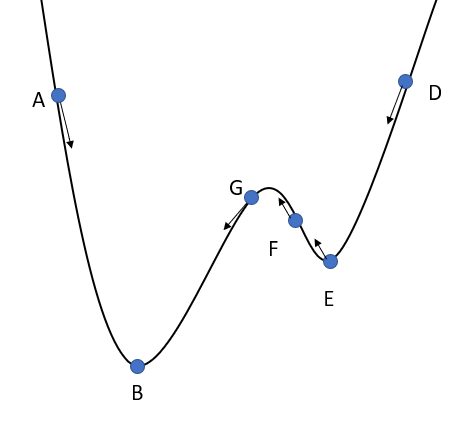
\includegraphics[scale=1]{chap2/image/momentum.png}
\caption{Đồ thị }
\end{center}
\end{figure}
Thuật toán gradient descent được ví như trọng lực tác dụng vào viên bi giúp nó di chuyển, B được coi điểm global minimum và E là một điểm local minimun. Để tránh hiện tượng nghiệm của gradient descent rơi vào một điểm local minimum không mong muốn thì ta tác động thêm một lực giúp gradient descent có thể bật ra khỏi vị trí của local minimum, lực này gọi là đà (\textit{momentum}). Vì thế cách cập nhật $\theta$ sẽ thay được thay đổi một chút như sau:
\begin{itemize}
\item[] $v_t:= \beta v_{t-1} +\eta \nabla\theta_{t}$
\item[]  $ \theta_t:= \theta_{t-1} - v_t$
\end{itemize}
Với $t$ là bước lặp thứ \textit{t}, biến $v$ được khởi tạo bằng 0 và trong tối ưu $\beta$ được gọi là đà (\textit{momentum}) với giá trị thường là $0.9$.
%\begin{algorithm}[H]
%\label{alg:momentum}
%\caption{Momentum kết hợp mini-batch}
%\begin{algorithmic}[1]
%\REQUIRE Tập n quan sát (\textbf{X},\textbf{y})
%\REQUIRE $\theta=[\theta_1,\theta_2,...,\theta_m]$
%\REPEAT 
%\STATE Xáo trộn dữ liệu
%\STATE v:=0
%\FORALL {$i=1;i \leq N;i=i+k$}
%\STATE $\nabla \theta_i := -\sum^{i+k}_{j=i} \nabla_{\theta}f(\theta;\textbf{x}_j,y_j)$
%\STATE $\mathit{v := mu*v+ \eta \nabla\theta_i}$
%\STATE Chọn bước nhảy $\eta$
%\STATE Cập nhật $\theta := \theta - v$
%\STATE if(hội tụ)
%\STATE break
%
%\ENDFOR
%
%\UNTIL	thuật toán hội tụ
%\end{algorithmic} 
%\end{algorithm}

\subsection{RMSprop}
\textit{RMSprop} là một cách giúp cho learning rate có thể thích nghi, điều chỉnh dựa trên độ lớn của gradient, được đưa ra bởi Geoff Hinton. Thuật toán này là một cách khắc phục việc dừng huấn luyện quá sớm khi áp dụng thuật toán Adagrad bằng cách chia learning rate cho . Khi áp dụng RMSprop, learning rate sẽ được thay đổi như sau:
\begin{itemize}
\item[] $m_t := \beta m_{t-1} + (1-\beta) \nabla\theta_{t}^2  $
\item[] $\theta_t := \theta_{t-1} - \frac{\eta}{\sqrt{m_{t-1}}+\epsilon}\nabla\theta_{t}$
\end{itemize}
Ta có biến $m$ được khởi tạo bằng 0 và $\beta$ là tốc độ giảm của learning rate, thường có giá trị là 0.9, 0.95 hoặc 0.99. Và $\epsilon$ giúp chúng ta tránh trường hợp chia cho 0, vì thế giá trị của $\epsilon$ thường là $10^{-8}$ 
\subsection{Adam}
\textit{Adam (Adaptive Moment Estimation)} là một bản cập nhật được đưa ra gần đây, nó khá giống với RMSprop và momentum. Cách cập nhật của thuật toán Adam như sau:
\begin{itemize}
\item[]  $m_t := \beta_1 m_{t-1} + (1-\beta_1) \nabla\theta_{t}$
\item[] $v_t := \beta_2 v_{t-1} + (1-\beta_2) \nabla\theta^2_{t}$
\item[] $ \widehat{m_t} := \frac{m_t}{1-\beta_1^{t}}$
\item[] $ \widehat{v_t} := \frac{v_t}{1-\beta_1^{t}} $
\item[] $\theta_t := \theta_1 + \frac{\eta }{\sqrt{\widehat{v_t}} +\epsilon}\widehat{m_t}$ 
\end{itemize}
$m_t,~v_t$ là giá trị ước lượng giữa thời điểm trước và thời điểm sau của các gradient tương ứng. Các giá trị của $m_t,~v_t$ đều được khởi tạo bằng 0. Các tác giả của Adam thấy rằng chúng bị lệch về 0, đặc biệt là các bước lặp đầu. Do vậy họ tạo ra $\widehat{m_t}~\text{và}~\widehat{v_t}$ để chống lại việc giá trị của $m_t ~\text{và}~ v_t$ lệch về 0. Các giá trị của $\beta_1,~\beta_2$ được tác giả đề xuất là 0.9 cho $\beta_1$, 0.999 cho $\beta2$  và $10^{-8} ~\text{cho}~ \epsilon$ như ở RMSprop.
